\section{Contact Conditions Between Particles}\label{sec:contact-conditions}

\begin{figure}
    \centering
    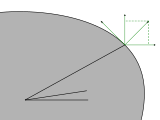
\includegraphics{img/model_development/node_shift_global}
    \caption{Geometric Conditions for Global Node Displacement}
    \label{fig:model_development/node_shift_global}
\end{figure}

In contrast to free surfaces, where the geometric evolution of a node is not constrained by the surrounding space, in grain boundaries the node shifting acts counter the solid material of the other particle.
This introduces additional constraints, since the grain boundary must not form voids and must not overlap.
The geometric constraints are dependent on the local evolution of the grain boundary nodes, as well as the relative position change of the particles.

Starting from a compact grain boundary, meaning that there are no holes and/or overlap present within it, the condition of maintaining the compactness of the grain boundary can be formulated as follows, if the postions of the particles are fixed.
\begin{subequations}
    \begin{align}
        \Step\Shift_{\Normal}\Regarding1 = \Step\Shift_{\Normal}\Regarding2 \\
        \Step\Shift_{\Tangential}\Regarding1 = \Step\Shift_{\Tangential}\Regarding2
    \end{align}
    \label{eq:maintain-compact-particles-fixed}
\end{subequations}

But in reality the positions of particles to each other change, which can be observed macroscopically as shrinkage.
So we formulate instead the total displacement of a node in absolute cartesian space, which must be equal regarded from both particles.
The total node displacement includes contributions from particle displacement (index $\Particle$), normal node displacement (index $\Normal$) and tangential node displacement (index $\Tangential$).
\begin{subequations}
    \begin{align}
        \Step\X_{\Particle1} + \Step\X_{\Normal}^{\Regarding1} + \Step\X_{\Tangential}^{\Regarding1} + \Step\X_{\RotationAngle}^{\Regarding1}
        &= \Step\X_{\Particle2} + \Step\X_{\Normal}^{\Regarding2} + \Step\X_{\Tangential}^{\Regarding2} + \Step\X_{\RotationAngle}^{\Regarding2}\\
        \Step\Y_{\Particle1} + \Step\Y_{\Normal}^{\Regarding1} + \Step\Y_{\Tangential}^{\Regarding1} + \Step\Y_{\RotationAngle}^{\Regarding1}
        &= \Step\Y_{\Particle2} + \Step\Y_{\Normal}^{\Regarding2} + \Step\Y_{\Tangential}^{\Regarding2} + \Step\Y_{\RotationAngle}^{\Regarding2}
        \label{eq:absolute-displacement-contact-constraints}
    \end{align}
\end{subequations}

As can be seen from \cref{fig:model_development/node_shift_global}, the angles of projection of the normal and tangential node shifting to the global cartesian axes are as follows:
\begin{subequations}
    \begin{align}
        \eta_{\Normal} &= \RotationAngle + \Angle + \left( \SurfaceRadiusAngle_{\Lower} + \SurfaceVectorAngle_{\Normal\Lower} - \PI \right)
        \label{eq:global-shift-normal-angle} \\
        \eta_{\Tangential} &= \left( \PI - \SurfaceRadiusAngle_{\Lower} + \SurfaceVectorAngle_{\Tangential\Lower} \right) - \RotationAngle - \Angle
        \label{eq:global-shift-tangential-angle}
    \end{align}
\end{subequations}

With these and further identities on the trigonometric functions the displacements of the node are given as follows:
\begin{subequations}
    \begin{align}
        \Step\X_{\Normal} &= -\Step\Shift_{\Normal} \cos \left( \RotationAngle + \Angle + \SurfaceRadiusAngle + \SurfaceVectorAngle \right)
        \label{eq:global-shift-normal-x} \\
        \Step\Y_{\Normal} &= -\Step\Shift_{\Normal} \sin \left( \RotationAngle + \Angle + \SurfaceRadiusAngle + \SurfaceVectorAngle \right)
        \label{eq:global-shift-normal-y} \\
        \Step\X_{\Tangential} &= \Step\Shift_{\Tangential} \cos \left( \RotationAngle + \Angle + \SurfaceRadiusAngle + \SurfaceVectorAngle \right)
        \label{eq:global-shift-tangential-x} \\
        \Step\Y_{\Tangential} &= \Step\Shift_{\Tangential} \sin \left( \RotationAngle + \Angle + \SurfaceRadiusAngle + \SurfaceVectorAngle \right)
        \label{eq:global-shift-tangential-y}
    \end{align}
\end{subequations}

Inserted in \cref{eq:absolute-displacement-contact-constraints} this leads to two additional constraints for each contact node (grain boundary or neck node), which define the particle displacements $\Step\X_{\Particle i}$ and $\Step\Y_{\Particle i}$ of each particle except one.
Given one grain boundary node (only normal displacement allowed) and two neck nodes per contact, the equation system is unambiguously defined as we have 6 additional constraints (2 per node) for 2 particle displacements and 4 tangential neck node displacements.
Introducing more grain boundary nodes creates more constraints but no additional unknowns (as their normal displacement and flux are covered by the volume balance respectively the optimization).
This leads to an overdetermined system which forces the solution to zero shrinkage (contact nodes are not able to be displaced at all).
Also allowing the grain boundary nodes to be displaced tangentially, leads to an underdetermined system as the contact conditions are not able to determine the particle position anymore.
A solution to this issue has not been found at the time writing this work, so the following applications will be restricted to two neck nodes and one grain boundary node per particle per contact.
This also forbids multiple contacts between the same particles, which is impossible for circular particle geometries but may be for arbitrarily shaped ones.
